%%% Lecture 1 Slides %%%

\documentclass{beamer}

%\documentclass[handout]{beamer}
%\usepackage{pgfpages}
%\pgfpagesuselayout{2 on 1}[a4paper,border shrink=5mm]
%\pgfpagesuselayout{1 on 1}[a4paper,border shrink=5mm]



\usepackage{amssymb}
\usepackage{amsmath}
\usepackage{mathtools}
\usepackage{tikz}
\usetikzlibrary{shapes,arrows}
\usetikzlibrary{positioning}
\usetikzlibrary{trees}
\usepackage{pgfplots}
\usepackage{pdflscape}
\usepackage{graphicx}
\usepackage{colortbl}
\usepackage{listings}
\usepackage{adjustbox}
\usepackage{physics}

\DeclarePairedDelimiter{\ceil}{\lceil}{\rceil}

\newcommand{\bs}{\boldsymbol}
\newcommand{\mb}{\mathbf}
\newcommand{\indep}{{\bot\negthickspace\negthickspace\bot}}
\newcommand{\notindep}{{\bot\negthickspace\negthickspace\bot}{\negthinspace
  \negmedspace \negthickspace \negthickspace \diagup
  \;}}
  \newcommand{\inred}[1]{\textcolor[RGB]{248,118,109}{#1}}
\newcommand{\ingreen}[1]{\textcolor[RGB]{0,191,196}{#1}}
\newcommand{\inblue}[1]{\textcolor{blue}{#1}}
\newcommand{\ind}[1]{1_{\{#1\}}}
\newcommand{\with}{\ingreen{\text{degree}}}
\newcommand{\without}{\inred{\text{no degree}}}

\renewcommand{\S}{\mb{S}}
\usepackage{color}
\definecolor{direct}{HTML}{FF0000}
\definecolor{indirect}{HTML}{FF9999}
\definecolor{dirin}{HTML}{990000}
\definecolor{control}{HTML}{999999}
\definecolor{directE}{HTML}{ED1C24}
\definecolor{indirectE}{HTML}{F69679}
\definecolor{controlE}{HTML}{999999}

%\def\V{{\rm V}\,}
\def\E{{\rm E}\,}
\def\arg{{\rm arg}\,}
\def\Cov{{\rm Cov}\,}
\def\N{{\rm N}\,}
\newcommand{\plim}{{\rm plim} \,}
\DeclareMathOperator*{\argmin}{arg\,min}
\newcommand{\X}{\mathbf{X}}
\newcommand{\Y}{\mathbf{Y}}
\newcommand{\Z}{\mathbf{Z}}
\newcommand{\I}{\mathbf{I}}
\newcommand{\V}{\mathbf{\Omega}}
\newcommand{\W}{\mathbf{W}}
\newcommand{\R}{\mathbf{R}}
\newcommand{\A}{\mathbf{A}}
\newcommand{\B}{\mathbf{B}}
\newcommand{\D}{\mathbf{D}}
\newcommand{\T}{\mathbf{T}}
\newcommand{\F}{\mathbf{F}}
\renewcommand{\O}{\mathbf{O}}
\renewcommand{\H}{\mathbf{H}}
\newcommand{\g}{\mathbf{g}}
\renewcommand{\r}{\mathbf{r}}
\newcommand{\s}{\mathbf{s}}
\newcommand{\uu}{\mathbf{u}}
\newcommand{\w}{\mathbf{w}}
\newcommand{\x}{\mathbf{x}}
\newcommand{\vv}{\mathbf{v}}
\newcommand{\z}{\mathbf{z}}
\newcommand{\y}{\mathbf{y}}

\newcommand{\bi}{\begin{itemize}}
\newcommand{\ei}{\end{itemize}}
\newcommand{\be}{\begin{enumerate}}
\newcommand{\ee}{\end{enumerate}}

\newcommand{\Beta}{\boldsymbol{\beta}}
\newcommand{\btheta}{\boldsymbol{\theta}}
\newcommand{\bgamma}{\boldsymbol{\gamma}}
\newcommand{\bpi}{\boldsymbol{\pi}}
\newcommand{\arrowp}{\stackrel{p}{\rightarrow}}
\newcommand{\arrowd}{\stackrel{d}{\rightarrow}}
\newcommand{\0}{\mathbf{0}}
\newcommand{\bP}{\mathbf{P}}
\newcommand{\nn}{\nonumber}
\def\S{{\sigma}}
\def\Supp{{\rm Supp}\,}


\newcommand\independent{\protect\mathpalette{\protect\independenT}{\perp}}
\def\independenT#1#2{\mathrel{\rlap{$#1#2$}\mkern2mu{#1#2}}}

\newcommand{\vsf}{\vspace{.5cm}}

\usepackage[english]{babel}
% or whatever

\usepackage[latin1]{inputenc}
% or whatever

\usepackage{times}
\usepackage[T1]{fontenc}
\setbeamertemplate{footline}[page number]{}
\setbeamertemplate{navigation symbols}{}


\title[Lecture 6: Causal Inference with a Binary Treatment] % (optional, use only with long paper titles)
{Lecture 6: Causal Inference with a Binary Treatment}


\begin{document}

\begin{frame}
  \titlepage
\end{frame}



\frame{
\frametitle{Review}

\begin{itemize}
\item Last lecture, we discussed learning subpopulation means and differences between subpopulation means based on a random sample (with replacement) from the population. \pause
\item Returning to the CPS example, we will consider 4-year degree holder incomes and income differences between 4-year degree holders and those without a 4-year degree. \pause
\item Even when the overall sample size is fixed (2246 for our example), different random samples will produce different subgroup sample sizes, and this adds a layer of complexity.  \pause
\item This complexity will not complicate our analysis much but it does complicate the justification for the analysis.
\end{itemize}

}

\begin{frame}{Agenda}

\begin{itemize}
\item Introduce formal causal inference with potential outcomes.
\item Demonstrate the identification of average treatment effects with randomized treatment assignment. 
%\item Discuss the relationship between the potential outcomes approach and the approach we have been using so far.
\item Discuss constant vs nonconstant treatment effects.
\end{itemize}

\end{frame}



\frame{
\frametitle{What is formal causal inference?}


\begin{itemize}
\item The formal approach reframes the problem of causal inference in terms of counterfactuals which are treated as missing data.  
\item This is a natural extension to sampling from populations where the unsampled portion of the population is treated as missing data. 
%\item The counterfactual approach can be seen as an extension of the model based approach we have taken so far in this course.
\item This reframing has lead to a revolution in the empirical sciences. 
\end{itemize}

}

\frame{
Optional readings for those interested: \\

\bigskip

\small


1. \small Angrist, Joshua D. and JornSteen Pischke (2010) \emph{The Credibility Revolution in Empirical Economics: How Better Research Design is Taking the Con out of Econometrics}, Journal of Economic Perspectives \pause \\

2.\\

\includegraphics[scale=.35]{figs/BookOfWhy}


}

\frame{
\frametitle{Potential Outcomes and Treatment Effects}


%Using the notation from Wooldridge Ch. 2.7a,\\
%\bigskip 

\begin{itemize}
\item $Y$ is an outcome variable (e.g. alive/dead, wages, etc.)
\item $D$ is a treatment variable (e.g. Treatment/Control, college degree/no degree)
\end{itemize} \pause

\vspace{.5cm}

Potential Outcomes: \\
$Y_i(1)$ is the potential outcome for individual $i$ if $D_i=1$. \\ \pause
$Y_i(0)$ is the potential outcome for individual $i$ if $D_i=0$. \\ \pause


\vspace{.5cm}

Treatment Effects:\\
For example, if patient $i$ will die without the treatment ($Y_i(0)=0$), but will live with the treatment ($Y_i(1)=1$), then the treatment effect for individual $i$ is
\begin{align*}
\tau_i &= Y_i(1) - Y_i(0)\\
 &= 1-0 \\
 &= 1
\end{align*}
}



\frame{
\frametitle{Illustrative Example}


Suppose we have six adult ADHD patients at a clinic. Two are being treated with stimulants ($D=1$) and four not ($D=0$). We are interested in the potential side effects of this treatment on resting heart rate ($Y$).

\begin{center}
\begin{tabular}{ccc|ccc}
$i$ & $D_i$ & $Y_i$ & $Y_i(1)$ & $Y_i(0)$ & $\tau_i=Y_i(1)-Y_i(0)$ \\
\hline
1 & 1 & 70 & 70 & \alert{?} & \alert{?} \\
2 & 1 & 80 & 80 & \alert{?} & \alert{?} \\
3 & 0 & 60 & \alert{?} & 60 & \alert{?} \\
4 & 0 & 70 & \alert{?} & 70 & \alert{?} \\
5 & 0 & 70 & \alert{?}& 70 & \alert{?} \\
6 & 0 & 80 & \alert{?} & 80 & \alert{?} \\
\end{tabular}
\end{center}


}


\frame{
\frametitle{Observed Outcomes vs Potential outcomes} 

\begin{align*}
Y_i &= (1-D_i)Y_i(0) + D_i Y_i(1)
\end{align*}

Illustrative Example (\alert{red numbers unknown}):
\begin{center}
\begin{tabular}{ccc|ccc}
$i$ & $D_i$ & $Y_i$ & $Y_i(1)$ & $Y_i(0)$ & $\tau_i$ \\
\hline
1 & 1 & 70 & 70 & \alert{70} & \alert{0} \\
2 & 1 & 80 & 80 & \alert{70} & \alert{10} \\
3 & 0 & 60 & \alert{70} & 60 & \alert{10} \\
4 & 0 & 70 & \alert{80} & 70 & \alert{10} \\
5 & 0 & 70 & \alert{70} & 70 & \alert{0} \\
6 & 0 & 80 & \alert{80} & 80 & \alert{0} \\
\end{tabular}
\end{center}

\emph{While $D$ affects $Y$, it does not affect $Y_i(1)$ or $Y_i(0)$!}

}




\frame{
\frametitle{Illustrative Example: Randomized Experiment}

Suppose the subjects were randomly assigned to $D=0$ and $D=1$ (also imagine these six subjects actually represent 600 subjects).
\begin{center}
\begin{tabular}{ccc|ccc}
$i$ & $D_i$ & $Y_i$ & $Y_i(1)$ & $Y_i(0)$ & $\tau_i$ \\
\hline
1 & 1 & 70 & 70 & \alert{70} & \alert{0} \\
2 & 1 & 80 & 80 & \alert{70} & \alert{10} \\
3 & 0 & 60 & \alert{70} & 60 & \alert{10} \\
4 & 0 & 70 & \alert{80} & 70 & \alert{10} \\
5 & 0 & 70 & \alert{70} & 70 & \alert{0} \\
6 & 0 & 80 & \alert{80} & 80 & \alert{0} \\
\end{tabular}
\end{center}

Randomization implies that $Y_i(1)$ and $Y_i(0)$ are independent of $D$, which implies that, 
\begin{align*}
E[Y_i(1)|D=1] &= E[Y_i(1)|D=0] = E[Y_i(1)]\\
E[Y_i(0)|D=1] &= E[Y_i(0)|D=0] = E[Y_i(0)]
\end{align*}

}

%\frame{
%\frametitle{Balance on Pre-treatment Variables in the Gerber, Green, and Larimer Experiment}
%
%\begin{center}
%
\includegraphics[width=4in]{GGL}
%\end{center}
%
%}

\frame{
\frametitle{Why Independence?}


\begin{center}
\begin{tabular}{ccc|ccc}
$i$ & $D_i$ & $Y_i$ & $Y_i(1)$ & $Y_i(0)$ & $\tau_i$ \\
\hline
1 & 1 & 70 & 70 & \alert{70} & \alert{0} \\
2 & 1 & 80 & 80 & \alert{70} & \alert{10} \\
3 & 0 & 60 & \alert{70} & 60 & \alert{10} \\
4 & 0 & 70 & \alert{80} & 70 & \alert{10} \\
5 & 0 & 70 & \alert{70} & 70 & \alert{0} \\
6 & 0 & 80 & \alert{80} & 80 & \alert{0} \\
\end{tabular}
\end{center}

With randomized treatment assignment,
\begin{itemize}
\item the $D=1$ rows are a random sample of the rows, therefore $E[Y_i(1)|D=1]= E[Y_i(1)] = E[Y_i(1)|D=0]$ % = E[Y_i(1)].   $E[y_i(1)|x=1] = E[y_i(1)]$ and $E[y_i(0)|x=1] = E[y_i(0)]$. 
\item the $D=0$ rows are a random sample of the rows, therefore $E[Y_i(0)|D=1] = E[Y_i(0)] = E[Y_i(0)|D=0]$  %E[y_i(1)|x=0] = E[y_i(1)]$ and $E[y_i(0)|x=0] = E[y_i(0)]$.
\end{itemize}

}

\frame{
\frametitle{Warning: Independence only for pre-treatment X}

\begin{itemize}
\item If $X$ is affected by $D$, then the previous results will not hold.
%\item Even though the $w=1$ rows are a random sample of the rows, $E[x|w=1] \ne E[x]$. 
%\item Even though the $w=0$ rows are a random sample of the rows, $E[x|w=0] \ne E[x]$.
%\item Therefore $E[x|w=1] \ne E[x|w=0]$.
\item Suppose $Y=1$ indicates a heart attack, $D=1$ is a blood pressure medicine, and $X$ is post-treatment blood pressure. $X$ will be affected by $D$ and will therefore not be independent of $D$
\end{itemize}

}



\frame{
\frametitle{$E[Y_i(1)]=E[Y_i(1)|D=1]=E[Y_i|D=1]$ and $E[Y_i(0)]=E[Y_i(0)|D=0]=E[Y_i|D=0]$}


Suppose subjects are randomly assigned to $D=0$ and $D=1$ (also imagine these six subjects actually represent 600 subjects).  

\begin{center}
\begin{tabular}{ccc|ccc}
$i$ & $D_i$ & $Y_i$ & $Y_i(1)$ & $Y_i(0)$ & $\tau_i$ \\
\hline
1 & 1 & 70 & 70 & \alert{70} & \alert{0} \\
2 & 1 & 80 & 80 & \alert{70} & \alert{10} \\
3 & 0 & 60 & \alert{70} & 60 & \alert{10} \\
4 & 0 & 70 & \alert{80} & 70 & \alert{10} \\
5 & 0 & 70 & \alert{70} & 70 & \alert{0} \\
6 & 0 & 80 & \alert{80} & 80 & \alert{0} \\
\end{tabular}
\end{center}

\visible<1-2>{What is the average $Y_i(1)$?} 
\visible<2>{$$
\frac{70 + 80 +\alert{70} + \alert{80} +\alert{70} + \alert{80}}{6}  = 75
$$}
\vspace{-2.4cm}

\visible<3-4>{What is the average $Y_i(1)$ among the $D=1$ subjects?} 
\visible<4>{$$
\frac{70 + 80 }{2}  = 75
$$}
\vspace{-2.4cm}

\visible<5-6>{What is the average $Y_i$ among the $D=1$ subjects?} 
\visible<6>{$$
\frac{70 + 80 }{2}  = 75
$$}
\vspace{-2.4cm}


\visible<7-8>{What is the average $Y_i(0)$?} 
\visible<8>{$$
\frac{\alert{70} +\alert{70} +60+ 70 +70 + 80}{6}  = 70
$$}

\vspace{-2.4cm}

\visible<9-10>{What is the average $Y_i(0)$ among the $D=0$ subjects?} 
\visible<10>{$$
\frac{60+ 70 +70 + 80}{4}  = 70
$$}

\vspace{-2.4cm}

\visible<11-12>{What is the average $Y_i$ among the $D=0$ subjects?} 
\visible<12>{$$
\frac{60+ 70 +70 + 80}{4}  = 70
$$}

}

\frame{
\frametitle{The ATE is the Difference in Average Potential Outcomes}


Suppose subjects are randomly assigned to $D=0$ and $D=1$ (also imagine these six subjects actually represent 600 subjects).  

\begin{center}
\begin{tabular}{ccc|ccc}
$i$ & $D_i$ & $Y_i$ & $Y_i(1)$ & $Y_i(0)$ & $\tau_i$ \\
\hline
1 & 1 & 70 & 70 & \alert{70} & \alert{0} \\
2 & 1 & 80 & 80 & \alert{70} & \alert{10} \\
3 & 0 & 60 & \alert{70} & 60 & \alert{10} \\
4 & 0 & 70 & \alert{80} & 70 & \alert{10} \\
5 & 0 & 70 & \alert{70} & 70 & \alert{0} \\
6 & 0 & 80 & \alert{80} & 80 & \alert{0} \\
\end{tabular}
\end{center}

\visible<1-2>{What is the average $Y_i(1)$?} 
\visible<2>{$$
\frac{70 + 80 +\alert{70} + \alert{80} +\alert{70} + \alert{80}}{6}  = 75
$$}
\vspace{-2.4cm}


\visible<3-4>{What is the average $Y_i(0)$?} 
\visible<4>{$$
\frac{\alert{70} +\alert{70} +60+ 70 +70 + 80}{6}  = 70
$$}

\vspace{-2.4cm}

\visible<5-6>{What is the average $\tau_i = Y_i(1) - Y_i(0)$?} 
\visible<6>{$$
75-70 = \frac{\alert{0} + \alert{10} + \alert{10}+  \alert{10} +\alert{0} +\alert{0}}{6}  = 5
$$}

}

\frame{
\frametitle{The Expected SLR slope is the ATE with randomized $D$}

\begin{center}
\begin{tabular}{ccc|ccc}
$i$ & $D_i$ & $Y_i$ & $Y_i(1)$ & $Y_i(0)$ & $\tau_i$ \\
\hline
1 & 1 & 70 & 70 & \alert{70} & \alert{0} \\
2 & 1 & 80 & 80 & \alert{70} & \alert{10} \\
3 & 0 & 60 & \alert{70} & 60 & \alert{10} \\
4 & 0 & 70 & \alert{80} & 70 & \alert{10} \\
5 & 0 & 70 & \alert{70} & 70 & \alert{0} \\
6 & 0 & 80 & \alert{80} & 80 & \alert{0} \\
\end{tabular}
\end{center}

\begin{align*}
\beta_1 &= E[Y_i|D_i=1] - E[Y_i|D_i=0] \\
&= \frac{70 + 80 }{2} - \frac{60 + 70 +70 + 80 }{4}\\
&=  \frac{70 + 80 +\alert{70} + \alert{80} +\alert{70} + \alert{80}}{6} - \frac{\alert{70} +\alert{70} +60+ 70 +70 + 80}{6} \\
&= \frac{\alert{0} + \alert{10} + \alert{10}+  \alert{10} +\alert{0} +\alert{0}}{6}
\end{align*}


}

\frame{

How can we connect causal inference to the population/descriptive inference we have been doing?

\bigskip

\begin{itemize}
\item Clarify causal vs descriptive interpretations.
\item Distinguish sample vs population causal inference.
\item Derive the SLR model from the potential outcomes model.
\end{itemize}

}

\frame{
\frametitle{Interpretation of $\beta_1$ in a simple regression}

\begin{columns}
\begin{column}{.5\textwidth}
Causal:\\
\vspace{.4cm}
$\beta_1$ is the expected effect of an extra unit of D (e.g., year of education) on Y (e.g., wages).
\vspace{1cm}
\end{column}
\begin{column}{.5\textwidth}
Descriptive:\\
\vspace{.4cm}
$\beta_1$ is the expected difference in Y (e.g., wages) between two individuals that have a one unit difference in D (e.g., years of education).
\end{column}
\end{columns}
\vspace{.8cm}

\pause

If we had a census (the whole population), the descriptive interpretation would always be valid. The causal interpretation would only be valid in some circumstances.
}


\frame{
\frametitle{Descriptive (Association) vs Causal from Hernan and Robins}

\begin{center}
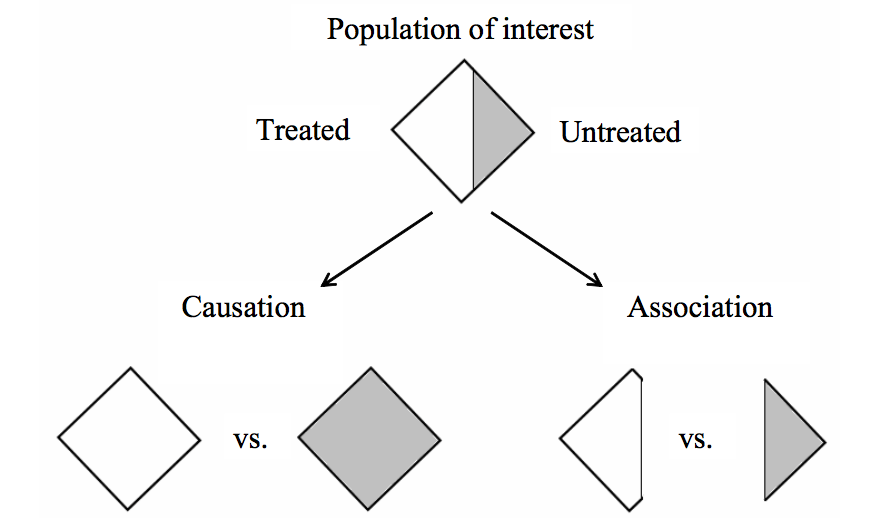
\includegraphics[width=4in]{figs/CvAnomath}
\end{center}


}

\frame{
\frametitle{Descriptive vs Causal and Sample vs Pop.}


\begin{center}
\begin{tabular}{ccc|ccc}
$i$ & $D_i$ & $Y_i$ & $Y_i(1)$ & $Y_i(0)$ & $\tau_i$ \\
\hline
1 & 1 & 70 & 70 & ? & ? \\
2 & 1 & 80 & 80 & ? & ? \\
3 & 0 & 60 & ? & 60 & ? \\
4 & 0 & 70 & ? & 70 & ? \\
5 & 0 & 70 & ? & 70 & ? \\
6 & 0 & 80 & ? & 80 & ? \\
\hline
7 & ? & ? & ? & ? & ? \\
8 & ? & ? & ? & ? & ? \\
\vdots & \vdots & \vdots & \vdots & \vdots & \vdots \\
\vdots & \vdots & \vdots & \vdots & \vdots & \vdots \\
%300 mil & ? & ? & ? & ? & ? \\
\end{tabular}
\end{center}


}


\frame{
\frametitle{Descriptive vs Causal and Sample vs Pop.}

\begin{center}
\begin{tabular}{ccc|ccc}
$i$ & $D_i$ & $Y_i$ & $Y_i(1)$ & $Y_i(0)$ & $\tau_i$ \\
\hline
\multicolumn{3}{c|}{Sample Descriptive Statistics} & \multicolumn{3}{c}{Sample Causal Inference} \\
\hline
1 & 1 & 70 & 70 & ? & ? \\
2 & 1 & 80 & 80 & ? & ? \\
3 & 0 & 60 & ? & 60 & ? \\
4 & 0 & 70 & ? & 70 & ? \\
5 & 0 & 70 & ? & 70 & ? \\
6 & 0 & 80 & ? & 80 & ? \\
\hline
\multicolumn{3}{c|}{Population Descriptive Inference} & \multicolumn{3}{c}{Population Causal Inference} \\
\hline
7 & ? & ? & ? & ? & ? \\
8 & ? & ? & ? & ? & ? \\
\vdots & \vdots & \vdots & \vdots & \vdots & \vdots \\
\vdots & \vdots & \vdots & \vdots & \vdots & \vdots \\
%300 mil & ? & ? & ? & ? & ? \\
\end{tabular}
\end{center}


}

\frame{
\frametitle{What does the ATE tell us?} 

Let's play CausalDoku! 
\begin{enumerate}
\item Randomization of $D$ implies (roughly) that the empty $Y_i(1)$ cells for $i=4,5,6$ must be filled with a 4 a 3 and a 2 (in some order)...
\item ...and the empty $Y_i(0)$ cells for $i = 1,2,3$ must be filled with a 3 and a 2 and a 1 (in some order).
\end{enumerate}

\begin{tabular}{ccc||c|c|c}
% Treatment & Outcome  & Outcome if Treated  & Outcome if Control  & Causal Effect  \\
$i$ & $D_i$ & $Y_i$ & $Y_i(1)$ & $Y_i(0)$ & $\tau_i=Y_i(1)-Y_i(0)$ \\
\hline
\hline
1&1 & 4 & 4 & &  \\
\hline
2&1 & 3 & 3 & & \\
\hline
3&1 & 2 & 2 & & \\
\hline
\hline
4&0 & 3 &   & 3 & \\
\hline
5&0 & 2 &   & 2 & \\
\hline
6& 0 & 1 &   & 1 & \\
\hline
\hline
\end{tabular}



}


\frame{
\frametitle{CausalDoku} 

Find two solutions:
\begin{enumerate}
\item with constant treatment effects
\item with both negative and positive effects
\end{enumerate}

\bigskip

\begin{tabular}{ccc||c|c|c}
% Treatment & Outcome  & Outcome if Treated  & Outcome if Control  & Causal Effect  \\
$i$ & $D_i$ & $Y_i$ & $Y_i(1)$ & $Y_i(0)$ & $\tau_i=Y_i(1)-Y_i(0)$ \\
\hline
\hline
1&1 & 4 & 4 & &  \\
\hline
2&1 & 3 & 3 & & \\
\hline
3&1 & 2 & 2 & & \\
\hline
\hline
4&0 & 3 &   & 3 & \\
\hline
5&0 & 2 &   & 2 & \\
\hline
6& 0 & 1 &   & 1 & \\
\hline
\hline
\end{tabular}

\bigskip

\pause

Note that both solutions imply the same ATE! 



}




\end{document}

